%\documentclass[handout,xcolor=pdftex,dvipsnames,table,mathserif]{beamer}
\documentclass[xcolor=pdftex,dvipsnames,table,mathserif]{beamer}
\usepackage{subfigure}
\usepackage{amsbsy}
\usepackage{tikz}
\usetikzlibrary{arrows}
\usepackage{amsmath,graphicx,dsfont,color}
\usepackage{amsfonts}
\usepackage{amssymb}
\usepackage{array}

\bibliographystyle{apalike}

\setbeamertemplate{bibliography item}{\insertbiblabel}
\setbeamertemplate{bibliography entry title}{}
\setbeamertemplate{bibliography entry location}{}
\setbeamertemplate{bibliography entry note}{}

%Definitiona

\newcommand{\x}{\mathbf{x}}
\newcommand{\X}{\mathbf{X}}
\newcommand{\W}{\mathbf{W}} %Weight
\newcommand{\bais}{\mathbf{b}}%Bais
\newcommand{\act}{\texttt{g}}%Activation
\newcommand{\loss}{L}
\newcommand{\pdata}{\hat{p}_{\texttt{data}}}
\newcommand{\nsize}{n}
\newcommand{\param}{\boldsymbol{\theta}}
\newcommand{\featmap}{\boldsymbol{\phi}}
\newcommand{\EV}{\mathbb{E}}







\usepackage{physics}

\graphicspath{{../graphics/}}

\AtBeginSection[]{
  \begin{frame}{Contents}
    \tableofcontents[currentsection, hideothersubsections]
  \end{frame}
}

\AtBeginSubsection[]{
  \begin{frame}{Contents}
    \tableofcontents[currentsection, subsectionstyle=show/shaded/hide]
  \end{frame}
}

\setbeamertemplate{footline}[frame number]{}
\setbeamertemplate{navigation symbols}{}
\setbeamertemplate{section in toc}[square]
\setbeamertemplate{items}[square]

%% For image credits on image bottom right
\usepackage[absolute,overlay]{textpos}
\setbeamercolor{framesource}{fg=gray}
\setbeamerfont{framesource}{size=\tiny}
\newcommand{\source}[1]{\begin{textblock*}{4cm}(8.7cm,8.6cm)
    \begin{beamercolorbox}[ht=0.5cm,right]{framesource}
      \usebeamerfont{framesource}\usebeamercolor[fg]{framesource} Credits: {#1}
    \end{beamercolorbox}
\end{textblock*}}

\title{Unsupervised anomalous image detection -- PhD thesis proposal}
\author{V. Machairas, E. Decencière}
\date{Capgemini Invent\\
  Mines Paris - PSL

}
\titlegraphic{
\includegraphics[height=2cm]{../graphics/logoemp}}

\useinnertheme{rounded}
\usecolortheme{rose}

%%%%%%%%%%%%%%%%%%%%%%%%%%%%%%%%%%%%%%%%%%%%%%%%%%%%%%%
%%%%%%%%%%%%%%%%%%%%%%%%%%%%%%%%%%%%%%%%%%%%%%%%%%%%%%%

\begin{document}

\frame{\titlepage}

\frame{
  \frametitle{Contents}
  \tableofcontents[hidesubsections]
}

%%%%%%%%%%%%%%%%%%%%%%%%%%%%%%%%%%%%%%%%%%%%%%%%%%
%%%%%%%%%%%%%%%%%%%%%%%%%%%%%%%%%%%%%%%%%%%%%%%%%%
\section{Introduction}

\begin{frame}{Diabetic retinopathy screening in fundus images}

  \begin{columns}
    \begin{column}{.5\textwidth}
  \begin{figure}[ht]
    \centering
    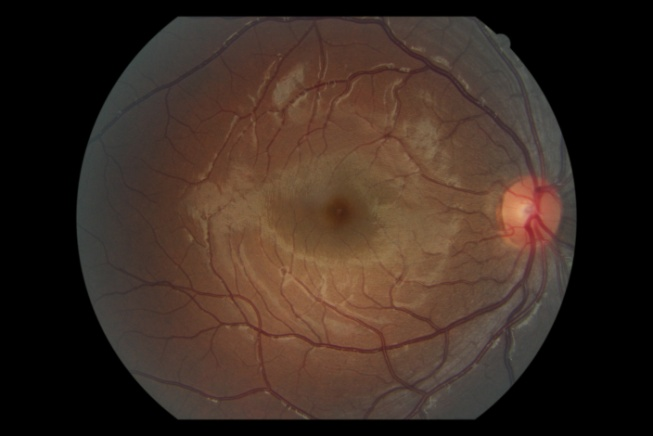
\includegraphics[width=\textwidth]{fundus1}
    \caption*{Normal image}
  \end{figure}

    \end{column}

    \begin{column}{.5\textwidth}

\begin{figure}[ht]
  \centering
  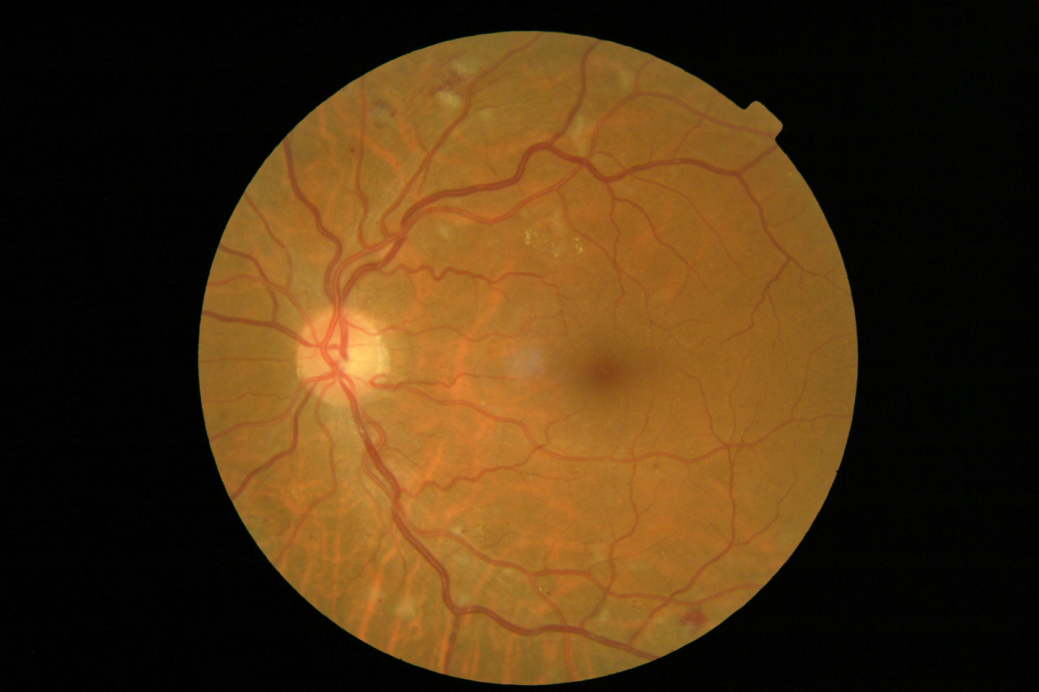
\includegraphics[width=\textwidth]{ret-dr}
  \caption*{Signs of diabetic retinopathy}
\end{figure}


    \end{column}
  \end{columns}

      \source{OPHDIAT database}

\end{frame}


%%%%%%%%%%%%%%%%%%%%%%%%%%%%%%%%%%%%
\begin{frame}{Unexpected case}

\begin{figure}[ht]
  \centering
  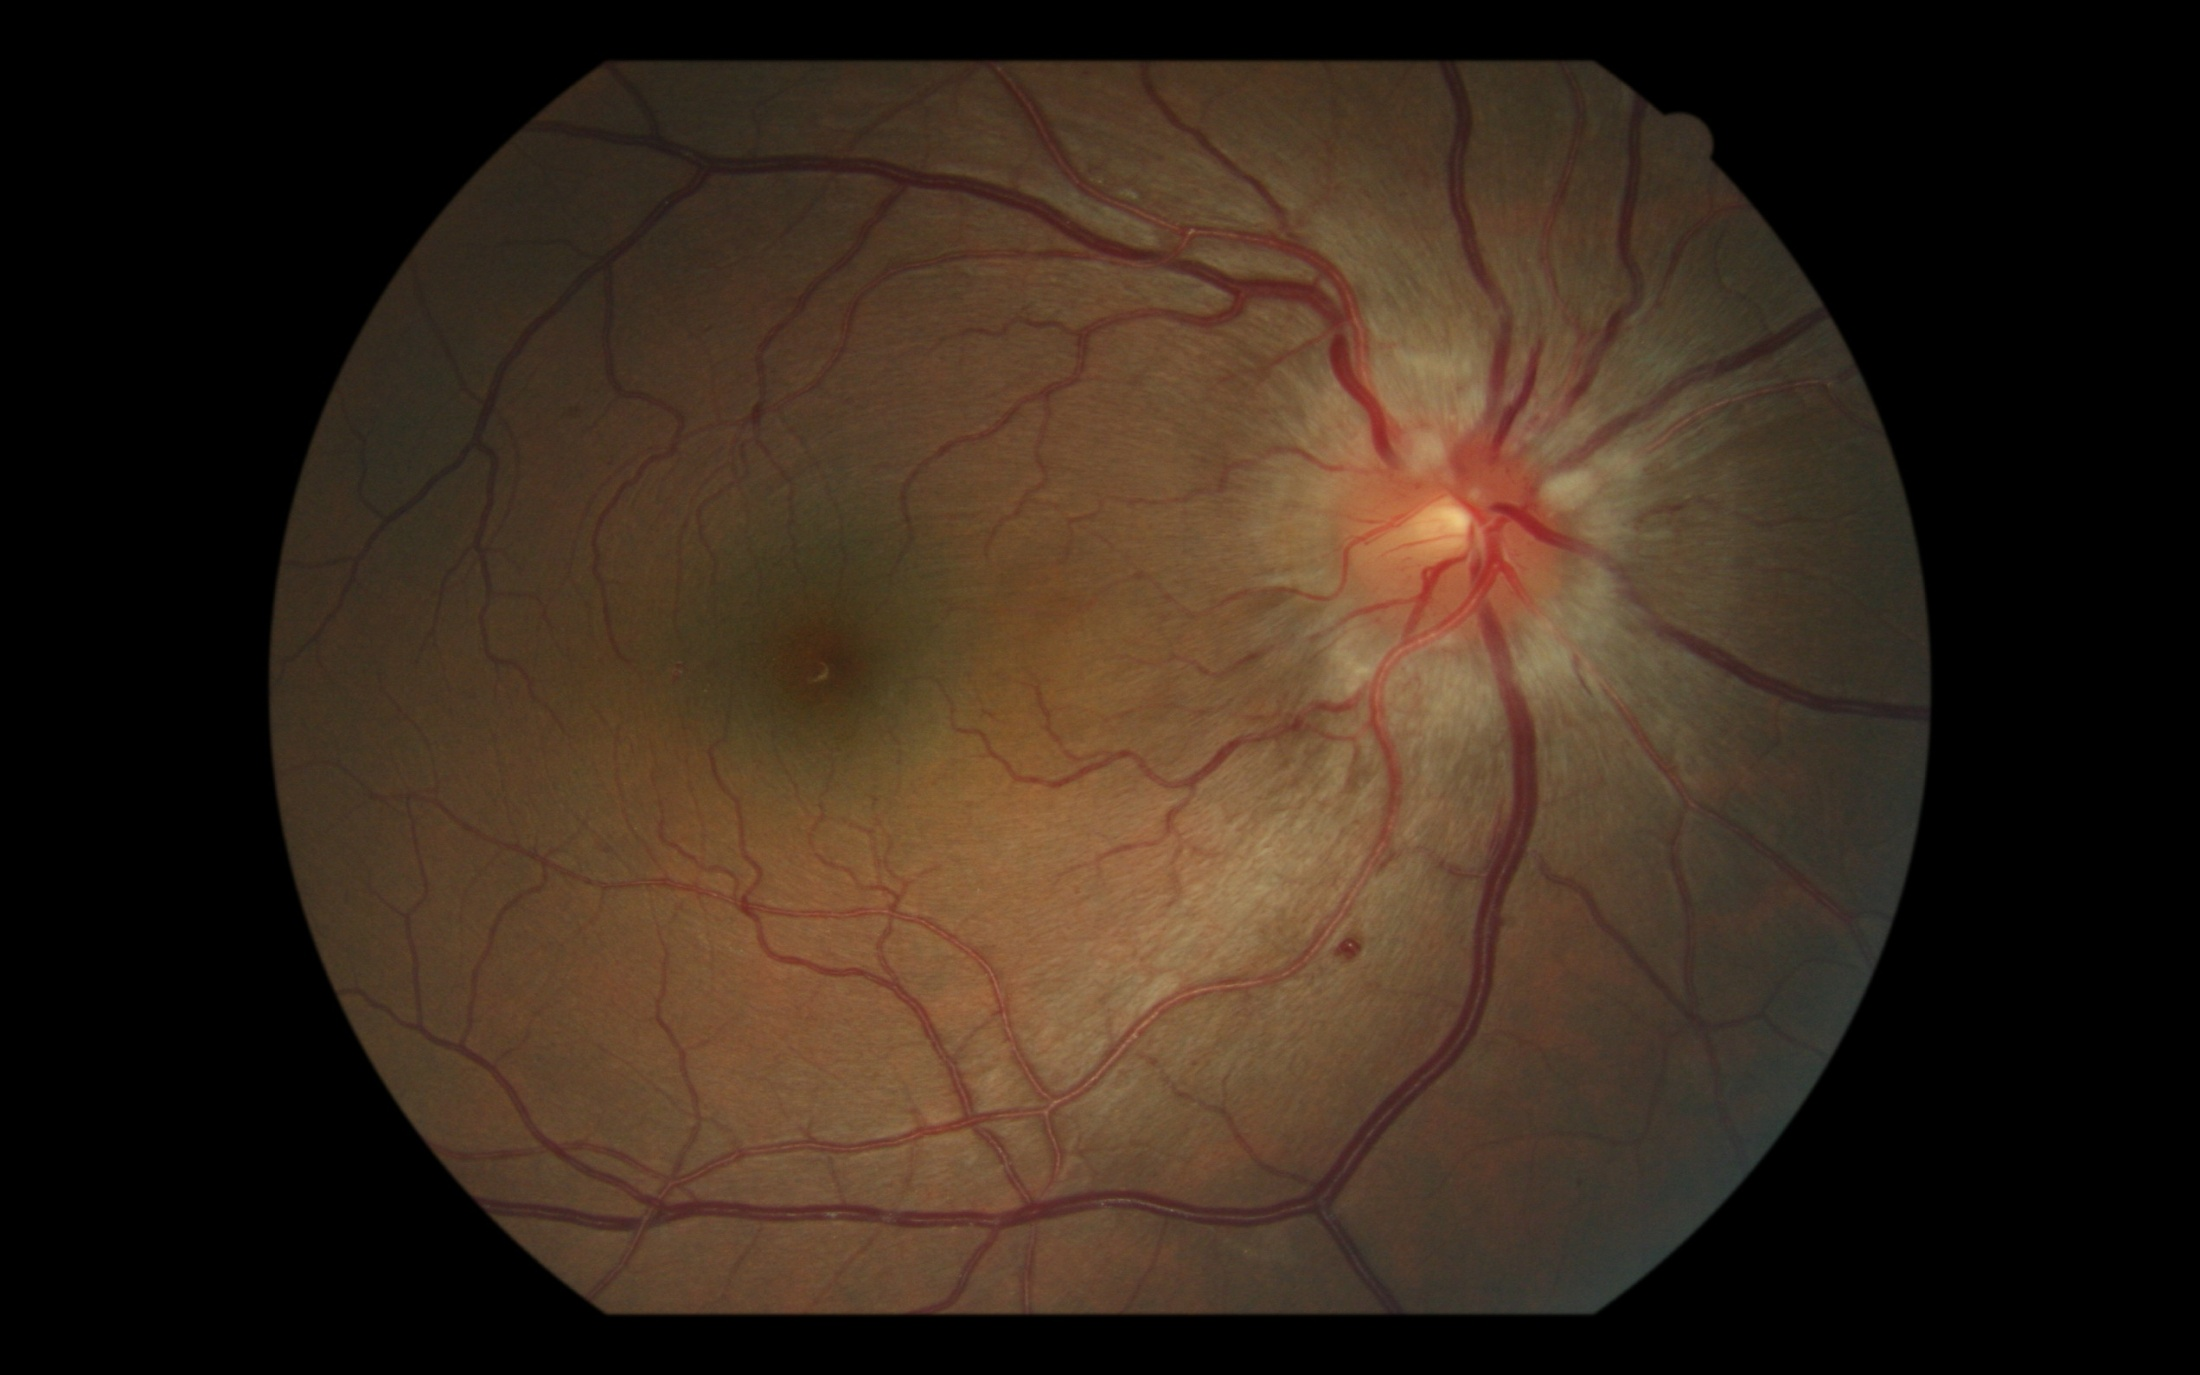
\includegraphics[width=0.6\textwidth]{ret-oedeme}
  \caption*{Papilledema}
\end{figure}


\end{frame}



%%%%%%%%%%%%%%%%%%%%%%%%%%%%%%%%%%%%
\begin{frame}{Anomalous image detection in a learning framework}

  \begin{block}{}
    \begin{itemize}
    \item Let us consider a given set of images. Among these, some  are defined as being \alert{normal}. The aim of the detection task is to decide, for any given image, if it is normal, or not.
    \item The definition of normal images is given through a set of examples.
    \end{itemize}
  \end{block}

  \begin{itemize}
  \item We will focus on images, but the problem is very general.
  \item We will suppose that we only have examples of normal images, i.e.\ that we are in a \alert{unsupervised} context. We assume that examples of anomalies are not representative enough or unknown.
  \end{itemize}

\end{frame}

%%%%%%%%%%%%%%%%%%%%%%%%%%%%%%%%%%%%
\begin{frame}{Vocabulary}

  \begin{itemize}
  \item Anomaly
  \item Novelty
  \item Outlier
  \end{itemize}

  In machine learning:

\begin{itemize}
\item One-class classification
\item Out-of-distribution (OOD) detection
\end{itemize}


\end{frame}


%%%%%%%%%%%%%%%%%%%%%%%%%%%%%%%%%%%%
\begin{frame}{Applications}

\begin{itemize}
\item Industrial control
\item Medicine, biology
\item Security
\item Astronomy
\end{itemize}

\vspace{1em}
\pause
\begin{block}{}
Anomaly detection is also a guardrail in applications where images are not systematically evaluated by a human eye.
\end{block}

\end{frame}


%%%%%%%%%%%%%%%%%%%%%%%%%%%%%%%%%%%%
\begin{frame}{MVTec~\tiny{\cite{bergmann_mvtec_2019}}}

\begin{itemize}
\item 15 categories
\item Training: 3629 (only normal images)
\item Testing: 1725
\end{itemize}

\begin{figure}[ht]
  \centering
  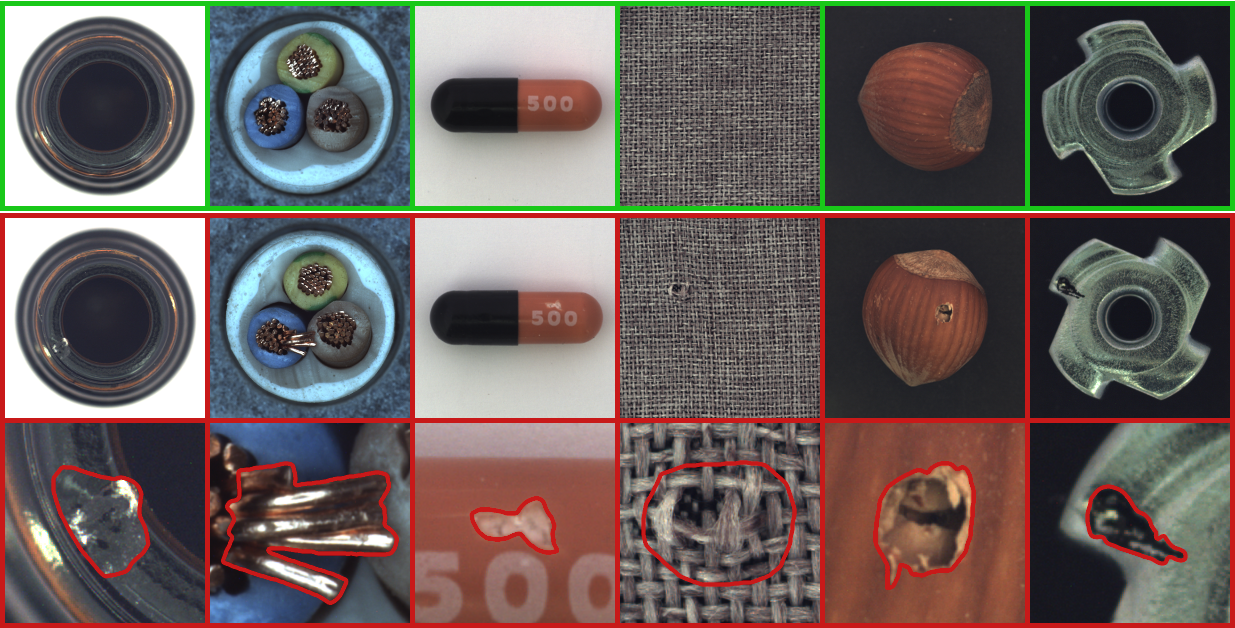
\includegraphics[width=0.8\textwidth]{mvtec}
\end{figure}

\end{frame}

%%%%%%%%%%%%%%%%%%%%%%%%%%%%%%%%%%%%
\begin{frame}{Visual Anomaly (VisA) Dataset~\tiny{\cite{zou_spot--difference_2022}}}

\begin{itemize}
\item 12 categories
\item 10821 high-resolution color images (9,621 normal and 1,200 anomalous)
\end{itemize}

\begin{figure}[ht]
  \centering
  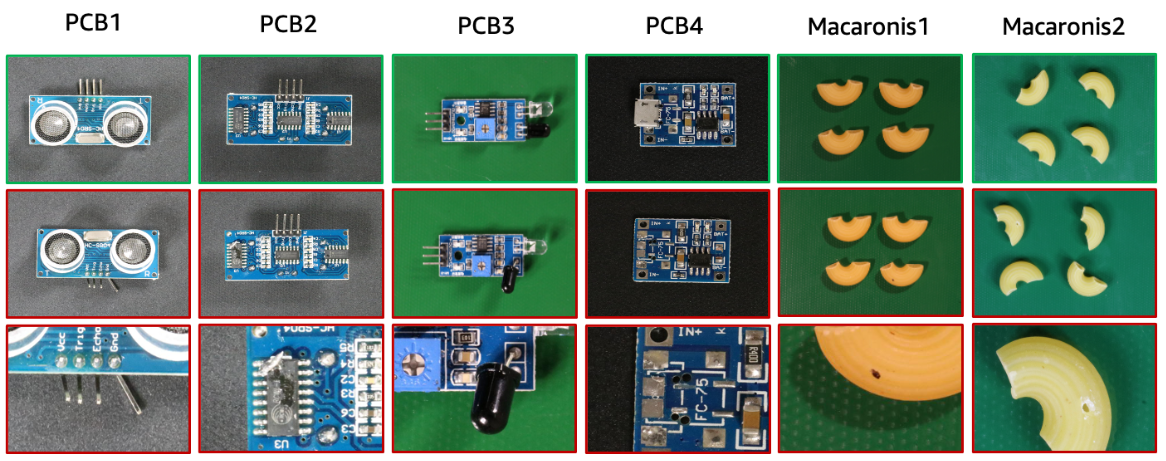
\includegraphics[width=0.8\textwidth]{visa}
\end{figure}

\end{frame}

%%%%%%%%%%%%%%%%%%%%%%%%%%%%%%%%%%%%
\begin{frame}{Retinal images}

  \begin{columns}
    \begin{column}{.5\textwidth}
  \begin{figure}[ht]
    \centering
    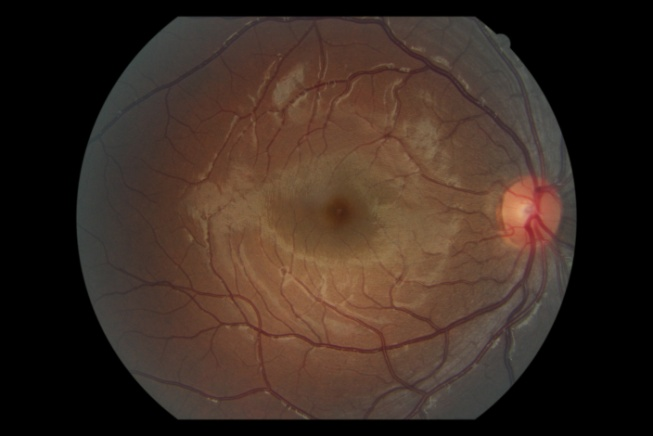
\includegraphics[width=\textwidth]{fundus1}
    \caption*{Normal image}
  \end{figure}

    \end{column}

    \begin{column}{.5\textwidth}

\begin{figure}[ht]
  \centering
  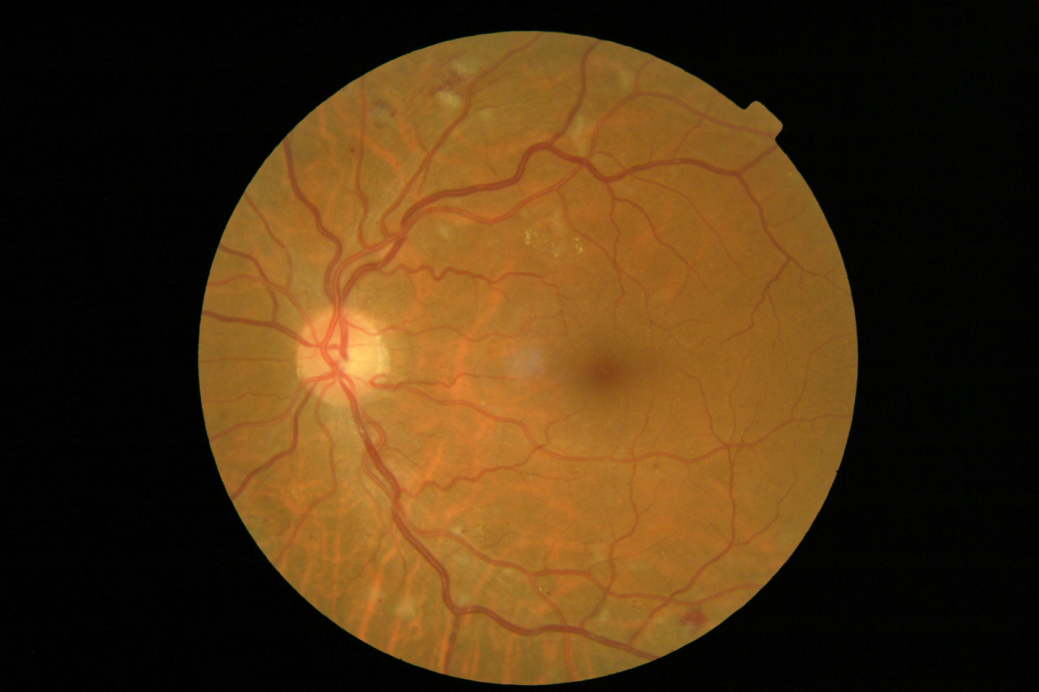
\includegraphics[width=\textwidth]{ret-dr}
  \caption*{Signs of diabetic retinopathy}
\end{figure}

    \end{column}
  \end{columns}



      \source{OPHDIAT database}

\end{frame}


%%%%%%%%%%%%%%%%%%%%%%%%%%%%%%%%%%%%
\begin{frame}{L'Oréal database}

Histological images of the skin, some of them containing anomalous tissues.

\end{frame}


%%%%%%%%%%%%%%%%%%%%%%%%%%%%%%%%%%%%
%% \begin{frame}{Evaluation}

%%   \begin{itemize}
%%   \item Classical methods
%%   \item AUPIMO (Joao C. Bertoldo)
%%   \end{itemize}

%% \end{frame}


%%%%%%%%%%%%%%%%%%%%%%%%%%%%%%%%%%%%%%%%%%%%%%%%%%
\section{State of the art}

%%%%%%%%%%%%%%%%%%%%%%%%%%%%%%%%%%%%
\begin{frame}{Major approaches}

  \begin{itemize}
  \item One-class classification
  \item Distillation methods
  \item Reconstruction methods
  \item Feature extraction
  \end{itemize}
\end{frame}


%%%%%%%%%%%%%%%%%%%%%%%%%%%%%%%%%%%%
\begin{frame}{One-class classification}

\begin{block}{Main idea}
To learn a compact classification of the normal data.
\end{block}

Examples:
\begin{itemize}
\item Estimating the support of a high dimensional distribution \cite{scholkopf_estimating_2001}
\item Deep one-class classification \cite{ruff_deep_2018}
\end{itemize}

\begin{figure}[ht]
  \centering
  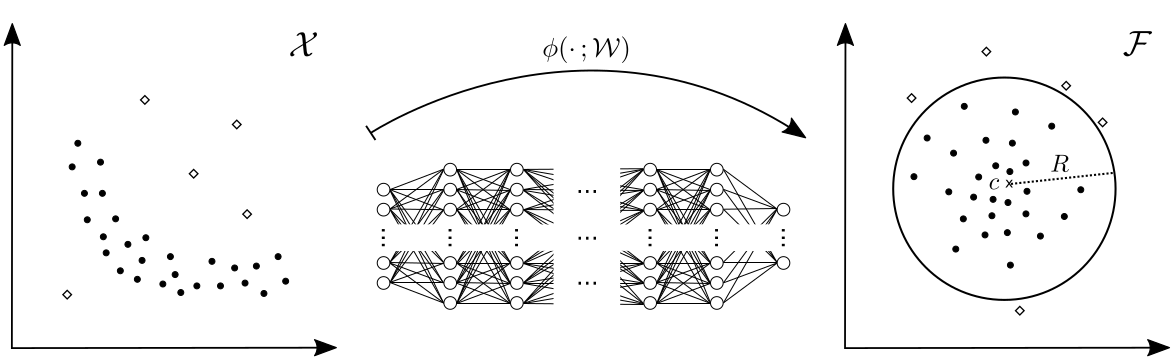
\includegraphics[width=0.8\textwidth]{deep_one_class_classifications}
\end{figure}

\end{frame}

%%%%%%%%%%%%%%%%%%%%%%%%%%%%%%%%%%%%
\begin{frame}{One-class classification}

\begin{block}{Conclusion}
  These methods run into severe difficulties when anomalous examples are not available.
\end{block}

\end{frame}


%%%%%%%%%%%%%%%%%%%%%%%%%%%%%%%%%%%%
\begin{frame}{Distillation methods}

\begin{block}{Main idea}
A small student networks is optimized to reproduce the behaviour of a large teacher network on normal samples. The discrepancy between these networks on anomalous samples is used to detect them.
\end{block}

Examples:
\begin{itemize}
\item Uninformed Students: Student-Teacher Anomaly Detection With Discriminative Latent Embeddings \cite{bergmann_uninformed_2020}
\end{itemize}

\end{frame}


%%%%%%%%%%%%%%%%%%%%%%%%%%%%%%%%%%%%
\begin{frame}{Distillation methods}

  \begin{block}{Conclusion}
    This relatively recent approach might be interesting. Further analysis is necessary before taking a decision.
  \end{block}
\end{frame}


%%%%%%%%%%%%%%%%%%%%%%%%%%%%%%%%%%%%
\begin{frame}{Reconstruction methods}

\begin{block}{Main idea}
An auto-encoder is optimized to reconstruct normal images. Anomalous images are expected to be incorrectly reconstructed.
\end{block}

Examples:
\begin{itemize}
\item Anomaly Detection Using Autoencoders with Nonlinear Dimensionality Reduction\cite{sakurada_anomaly_2014}
\item A Fast Method For Anomaly Detection And Segmentation \cite{ndiour_fre_2022}
\end{itemize}

\end{frame}

%%%%%%%%%%%%%%%%%%%%%%%%%%%%%%%%%%%%
\begin{frame}{Reconstruction methods}

  \begin{block}{Conclusion}
    This family of methods remains enticing, even if they do not reach state of the art results. Understanding their limits should help moving forward the state of the art. Furthermore, they can help building appropriate latent spaces.
  \end{block}
\end{frame}


%%%%%%%%%%%%%%%%%%%%%%%%%%%%%%%%%%%%
\begin{frame}{Feature extraction}

\begin{block}{Main idea}
To use a pretrained network on a large dataset and to characterize the distribution of normal representations in a latent space to detect anomalous ones.
\end{block}

Examples:
\begin{itemize}
\item Modeling the Distribution of Normal Data in Pre-Trained Deep Features for Anomaly Detection \cite{rippel_modeling_2020}
\begin{figure}[ht]
  \centering
  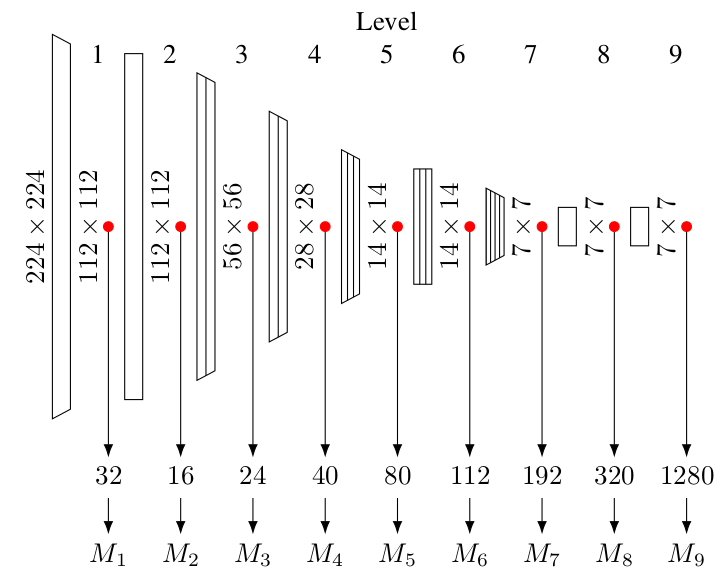
\includegraphics[width=0.35\textwidth]{enb0_features}
\end{figure}
\item PaDiM: A Patch Distribution Modeling Framework for Anomaly Detection and Localization \cite{defard_padim_2021}
\end{itemize}

\end{frame}

%%%%%%%%%%%%%%%%%%%%%%%%%%%%%%%%%%%%
\begin{frame}{Feature extraction}

\begin{block}{Conclusion}
   These methods are already quite competitive. Analysing and solving their limitations should be a promising research direction.
\end{block}

\end{frame}


%%%%%%%%%%%%%%%%%%%%%%%%%%%%%%%%%%%%
\begin{frame}{Other approaches}

\begin{itemize}
\item SimpleNet: A Simple Network for Image Anomaly Detection and Localization~\cite{liu_simplenet_2023}
\item On Diffusion Modeling for Anomaly Detection~\cite{livernoche_diffusion_2023}
\end{itemize}

  \begin{figure}[ht]
    \centering
    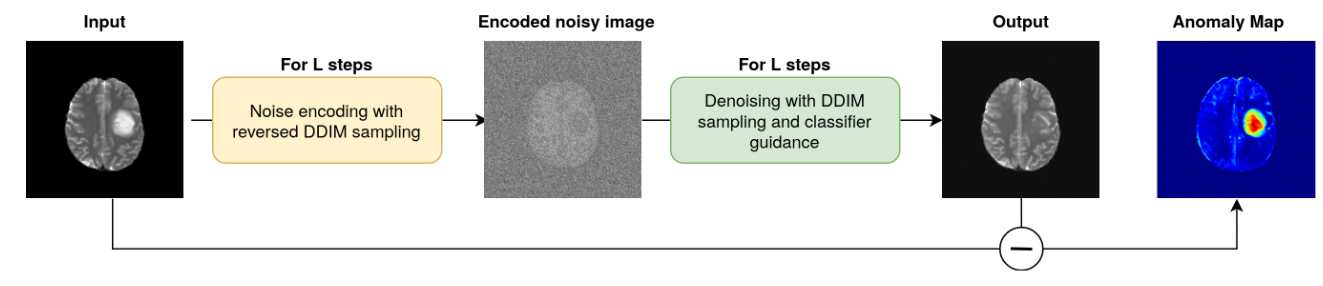
\includegraphics[width=\textwidth]{2022.miccai.wolleb}
    \cite{wolleb_diffusion_2022}
  \end{figure}


\end{frame}

%%%%%%%%%%%%%%%%%%%%%%%%%%%%%%%%%%%%
\begin{frame}{Limits of current approaches}

  \begin{figure}[ht]
    \centering
    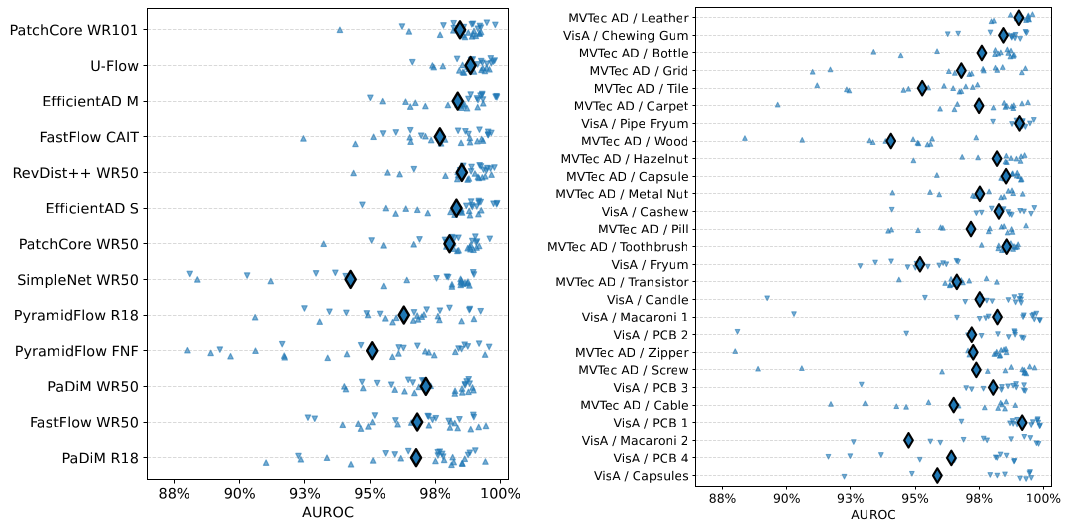
\includegraphics[width=\textwidth]{auroc_per_base_per_method}
  \end{figure}


\end{frame}




%%%%%%%%%%%%%%%%%%%%%%%
%%%%%%%%%%%%%%%%%%%%%%%
\section{Research project}

%%%%%%%%%%%%%%%%%%%%%%%%%%%%%%%%%%%%
\begin{frame}{Three steps}

  \begin{enumerate}
  \item Building an appropriate latent space
  \item Explore the latent space
  \item Reconstruction approaches
  \end{enumerate}

\end{frame}

%%%%%%%%%%%%%%%%%%%%%%%%%%%%%%%%%%%%
\begin{frame}{Building an appropriate latent space}

\begin{itemize}
\item Self-supervised learning for anomaly detection~\cite{langrognet_self-supervised_2025}
\item Comparison with ImageNet representations
\end{itemize}

\begin{block}{Risk-benefit balance}
  \hspace{4em} Risk : low \hspace{4em} Benefits : medium
\end{block}

\end{frame}

%%%%%%%%%%%%%%%%%%%%%%%%%%%%%%%%%%%%
\begin{frame}{Exploring the latent space}

\begin{itemize}
   \item Use the latent space built in the previous step
   \item Explore it using:
     \begin{itemize}
     \item Greedy direction selection~\cite{gula_gaussian_2023}
     \item Random noise (\textit{à la} SimpleNet)
     \end{itemize}
\end{itemize}

\begin{block}{Risk-benefit balance}
  \hspace{4em} Risk : medium \hspace{4em} Benefits : high
\end{block}

\end{frame}

%%%%%%%%%%%%%%%%%%%%%%%%%%%%%%%%%%%%
\begin{frame}{SimpleNet\tiny{\cite{liu_simplenet_2023}}}

  \begin{figure}[ht]
  \centering
  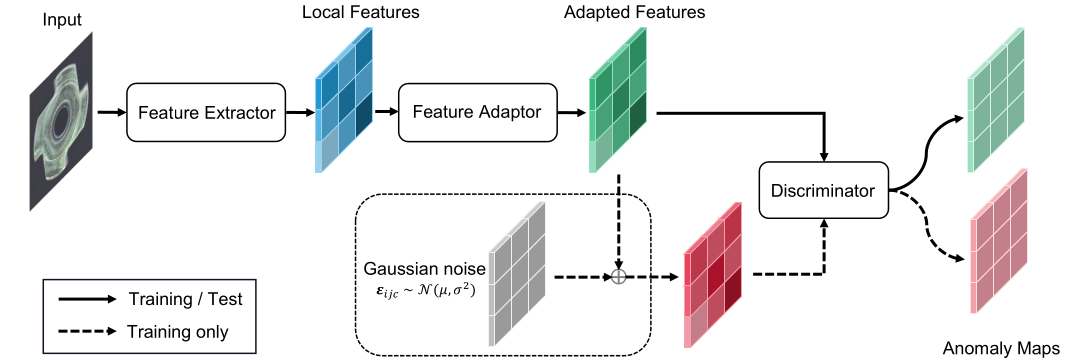
\includegraphics[width=0.9\textwidth]{simplenet}
\end{figure}

\end{frame}

%%%%%%%%%%%%%%%%%%%%%%%%%%%%%%%%%%%%
\begin{frame}{Reconstruction approaches}

\begin{itemize}
\item Use the latent space from the first part
\item Detect anomalies using a semantic-aware norm
\end{itemize}

\begin{block}{Risk-benefit balance}
\hspace{4em} Risk : high \hspace{4em} Benefits : high
\end{block}

\end{frame}


%%%%%%%%%%%%%%%%%%%%%%%%%%%%%%%%%%%%
\begin{frame}{Develop an application}


\end{frame}

%%%%%%%%%%%%%%%%%%%%%%%%%%%%%%%%%%%%
\begin{frame}{Dissemination}

  \begin{itemize}
  \item Publication in major research conferences and journals
  \item Code diffusion (with an appropriate open source licence)
  \end{itemize}

\end{frame}


%%%%%%%%%%%%%%%%%%%%%%%%%%%%%%%%%%%%%%%%%%%%%%%%%%
\section{Action plan}

%%%%%%%%%%%%%%%%%%%%%%%%%%%%%%%%%%%%
\begin{frame}{Action plan}

  \begin{itemize}
  \item Discuss scientific program
  \item General terms of the collaboration between Capgemini Invent and Mines Paris
    \begin{itemize}
    \item Contribution to our effort : 33 k€ / year
    \item IP : to be discussed, but we have to be able to continue our research missions on this subject beyond this project.
    \end{itemize}
  \item Write PhD proposal
  \item Write contract
  \item Only proceed if we find a candidate considered good by both parties
  \end{itemize}

\end{frame}


%%%%%%%%%%%%%%%%%%%%%%%%%%%%%%%%%%%%
\section{Supplementaries}

%%%%%%%%%%%%%%%%%%%%%%%%%%%%%%%%%%%%
\begin{frame}{Self-supervised learning with triplet loss}

\begin{figure}[ht]
  \centering
  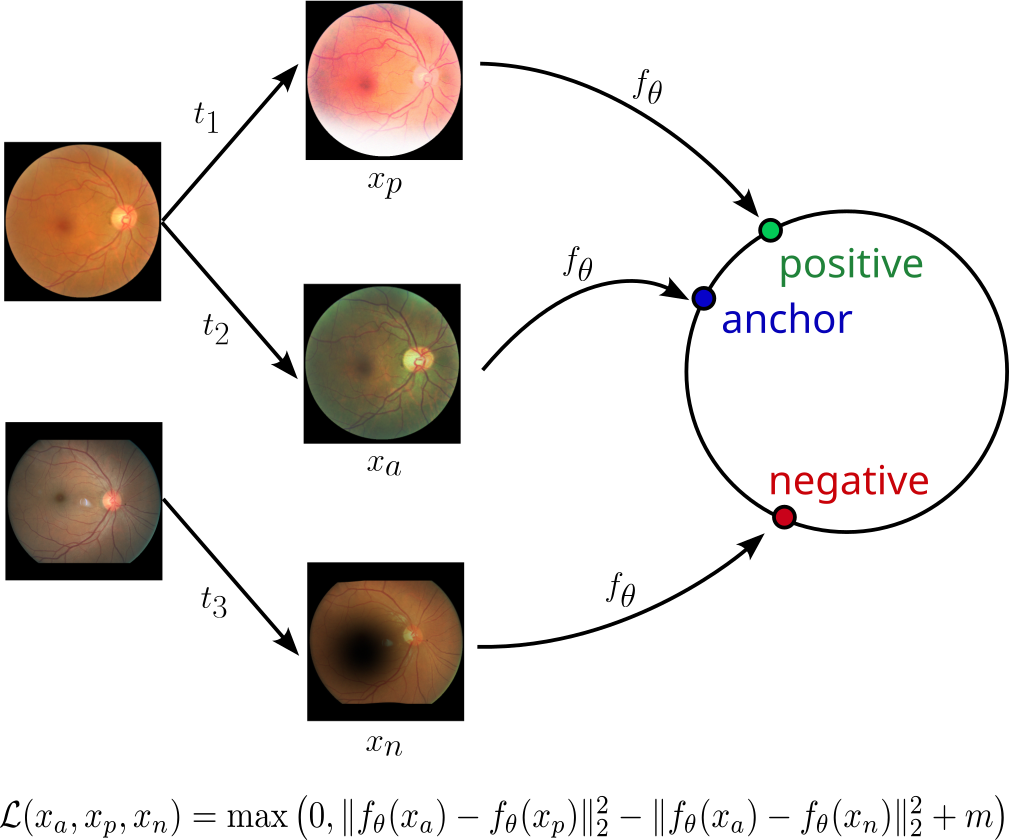
\includegraphics[width=0.7\textwidth]{ssl}
\end{figure}

\end{frame}


%%%%%%%%%%%%%%%%%%%%%%%%%%%%%%%%%%%%
\begin{frame}{Using the Mahalanobis distance in the latent space}

\begin{columns}
  \begin{column}{.5\textwidth}
  \begin{figure}[ht]
    \centering
    \includegraphics[width=\textwidth]{graphic_method_crop}
  \end{figure}

  \end{column}

  \begin{column}{.5\textwidth}
    \tiny
    \[S(x) = \sqrt{(f_{\theta}(x)-\hat{\mu}_h)^{T}\hat{\Sigma}^{-1}_{h} (f_{\theta}(x)-\hat{\mu}_h)}\]
  \end{column}
\end{columns}


\end{frame}


%%%%%%%%%%%%%%%%%%%%%%%%%%%%%%%%%%%%%%%%%%%%%%%%%%
\section*{References}

%%%%%%%%%%%%%%%%%%%%%%%%%%%%%%%%%%%%%%%%%%%%%%%%%%

\frame[allowframebreaks]{

  \scriptsize

  \frametitle{References}

  %\bibliographystyle{amsalpha}
  %\bibliographystyle{apalike}

  \bibliography{../../edf.bib}

  \normalsize

}




\end{document}
